\appendix

\chapter{Code} \label{python_code}

\section{Core project}
\paragraph*{Contains database management, data-processing and machine learning model creation}
\inputminted[linenos, fontsize=\tiny]{python}{code/fusion_file_appendix.py}
\clearpage

\section{Flickr mining script}
\inputminted[linenos, fontsize=\tiny]{python}{code/flickr_mining_Kt_Zug_Appendix.py}
\clearpage


\chapter{SQL queries for training data} \label{sql_queries_for_trainingdata}

\section{Class: walking}

\inputminted[linenos]{sql}{code/walking.txt}
\clearpage

\section{Class: hiking}

\inputminted[linenos]{sql}{code/hiking.txt}
\clearpage

\section{Class: jogging}

\inputminted[linenos]{sql}{code/jogging.txt}
\clearpage

\section{Class: biking}

\inputminted[linenos]{sql}{code/biking.txt}
\clearpage

\section{Class: dog walking}

\inputminted[linenos]{sql}{code/dog_walking.txt}
\clearpage

\section{Class: horse riding}

\inputminted[linenos]{sql}{code/horse_riding.txt}
\clearpage

\section{Class: picnic}

\inputminted[linenos]{sql}{code/picnic.txt}
\clearpage

%\chapter{Confusion matrix} \label{confusion_matrix}

%\chapter{Model validation tables} \label{model_validation_tables}

\chapter{Best M2 class-features} \label{M2_top_features}
\begin{figure}[h!]
   \centering
   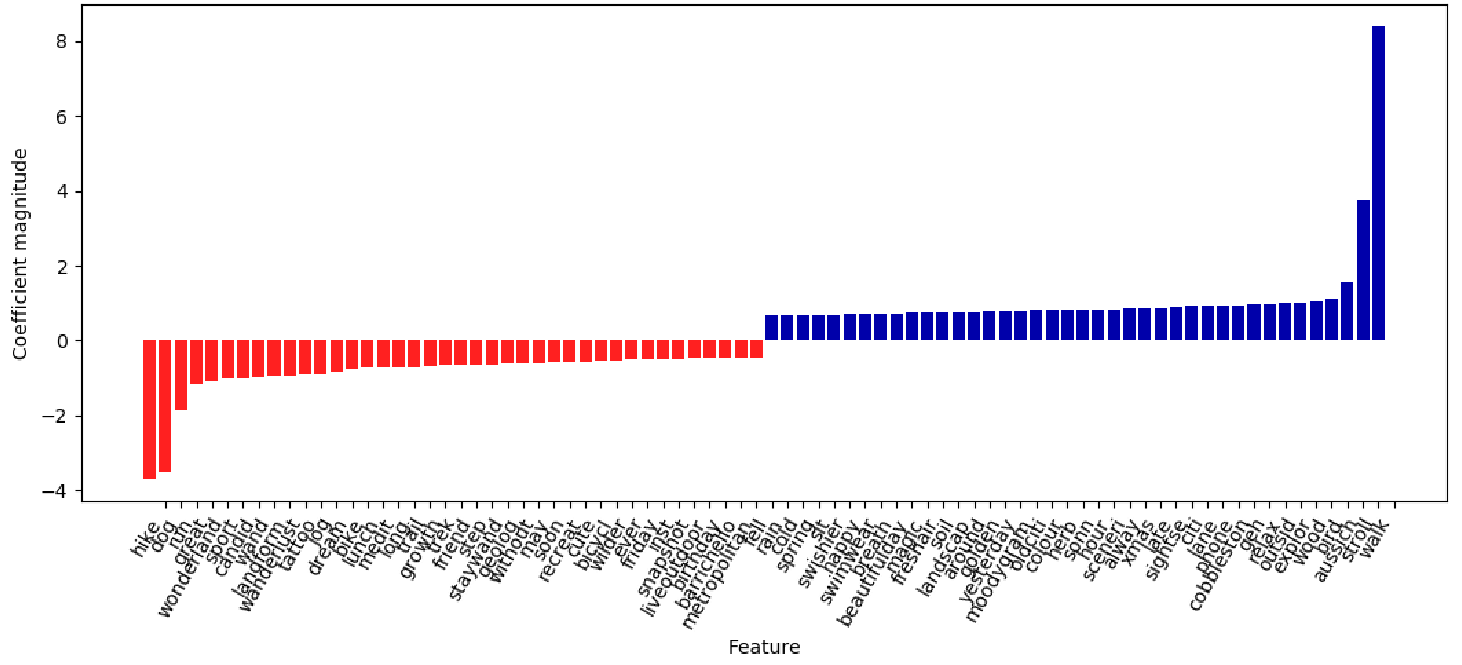
\includegraphics[width=\textwidth]{img/m2_top40_features_walking_cropped.pdf}
   \caption{The top 80 most predictive M2-features of the class 'walking'. Blue features are word-tokens which supports the presence of the corresponding classification. Red features support the opposite. The graphic was created with the \textit{mglearn} Python library provided by \textcite{Guido2016}}
   \label{fig:M2_top40_features_walking}
\end{figure}
\begin{figure}[h!]
   \centering
   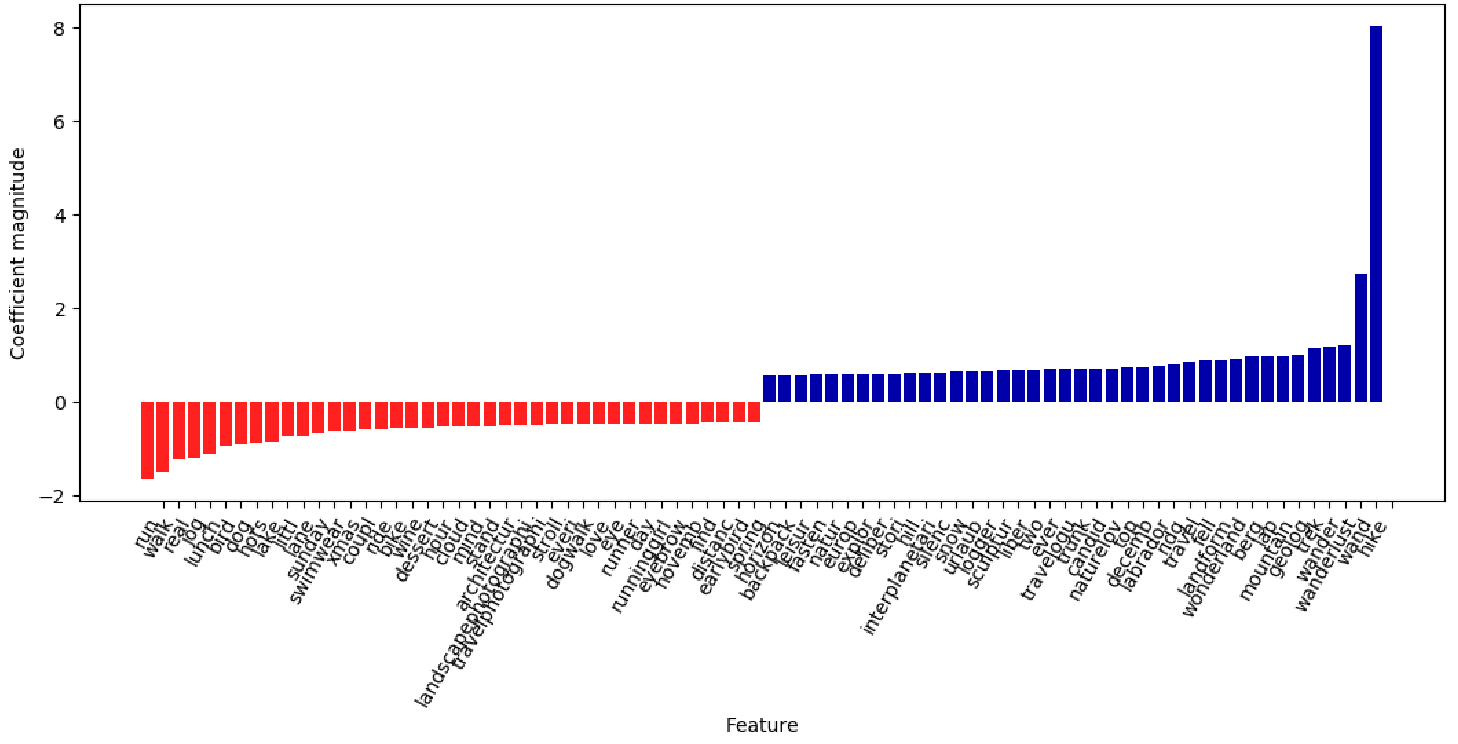
\includegraphics[width=\textwidth]{img/m2_top40_features_hiking_cropped.pdf}
   \caption{The top 80 most predictive M2-features of the class 'hiking'. Blue features are word-tokens which supports the presence of the corresponding classification. Red features support the opposite. The graphic was created with the \textit{mglearn} Python library provided by \textcite{Guido2016}}
   \label{fig:M2_top40_features_hiking}
\end{figure}
\begin{figure}[h!]
   \centering
   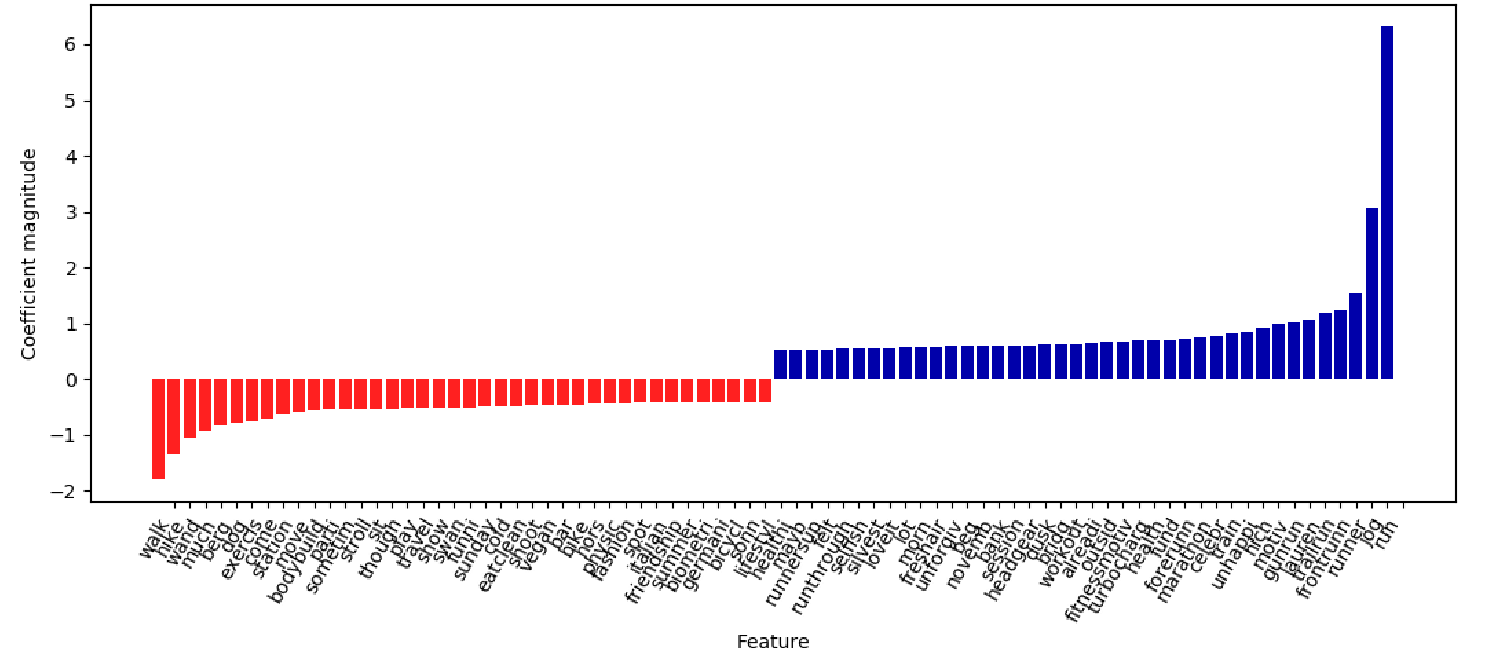
\includegraphics[width=\textwidth]{img/m2_top40_features_Jogging_cropped.pdf}
   \caption{The top 80 most predictive M2-features of the class 'jogging'. Blue features are word-tokens which supports the presence of the corresponding classification. Red features support the opposite. The graphic was created with the \textit{mglearn} Python library provided by \textcite{Guido2016}}
   \label{fig:M2_top40_features_jogging}
\end{figure}
\begin{figure}[h!]
   \centering
   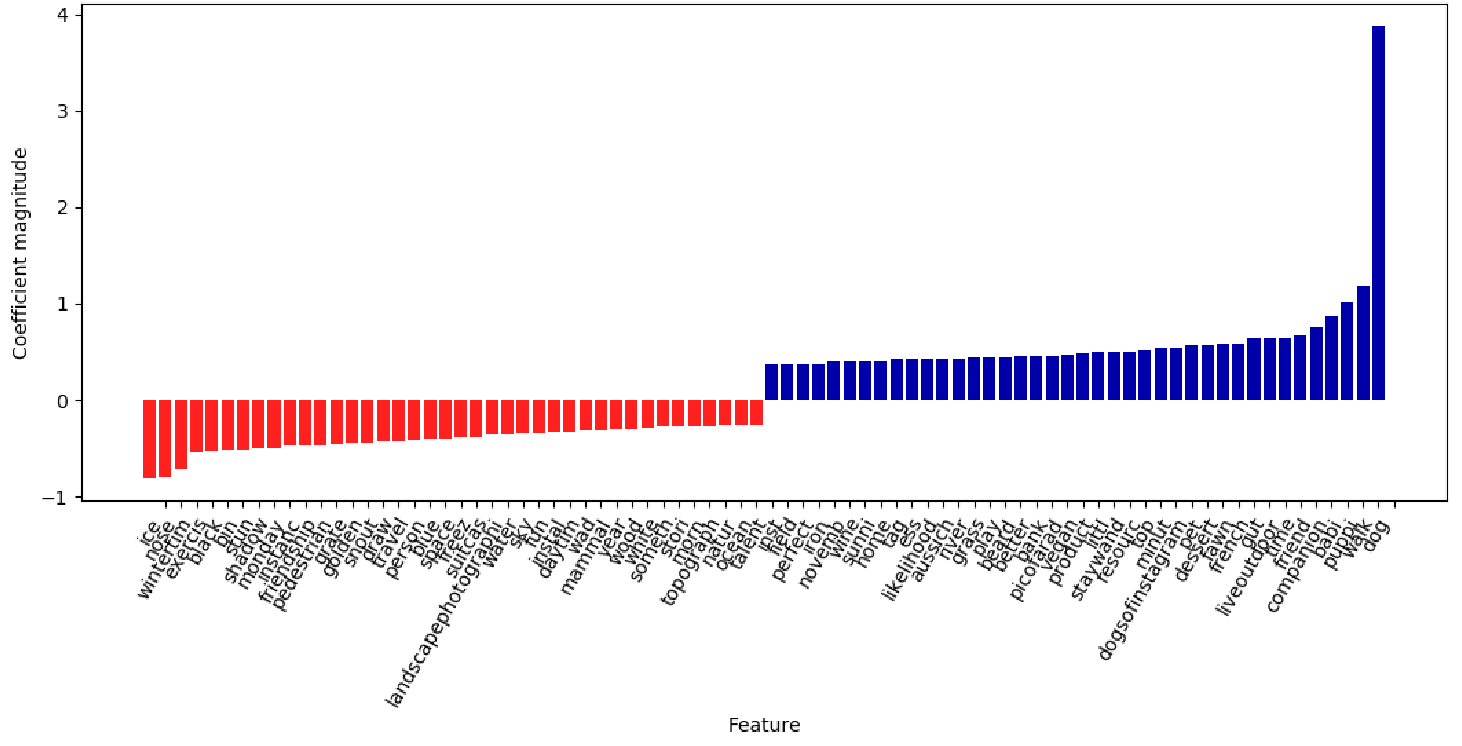
\includegraphics[width=\textwidth]{img/m2_top40_features_dog_walking_cropped.pdf}
   \caption{The top 80 most predictive M2-features of the class 'dog walking'. Blue features are word-tokens which supports the presence of the corresponding classification. Red features support the opposite. The graphic was created with the \textit{mglearn} Python library provided by \textcite{Guido2016}}
   \label{fig:M2_top40_features_dog_walking}
\end{figure}
\begin{figure}[h!]
   \centering
   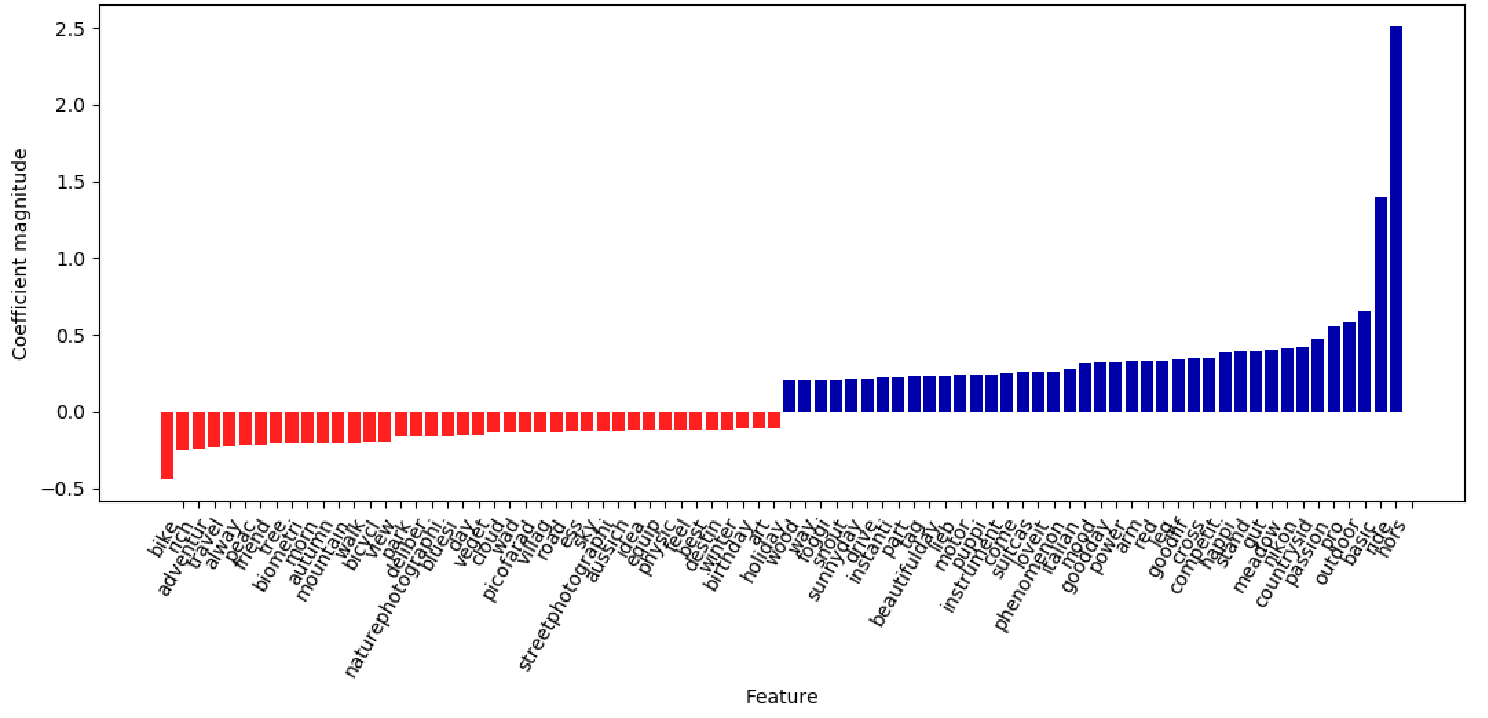
\includegraphics[width=\textwidth]{img/m2_top40_features_horse_riding_cropped.pdf}
   \caption{The top 80 most predictive M2-features of the class 'horse riding'. Blue features are word-tokens which supports the presence of the corresponding classification. Red features support the opposite. The graphic was created with the \textit{mglearn} Python library provided by \textcite{Guido2016}}
   \label{fig:M2_top40_features_horse_riding}
\end{figure}
\begin{figure}[h!]
   \centering
   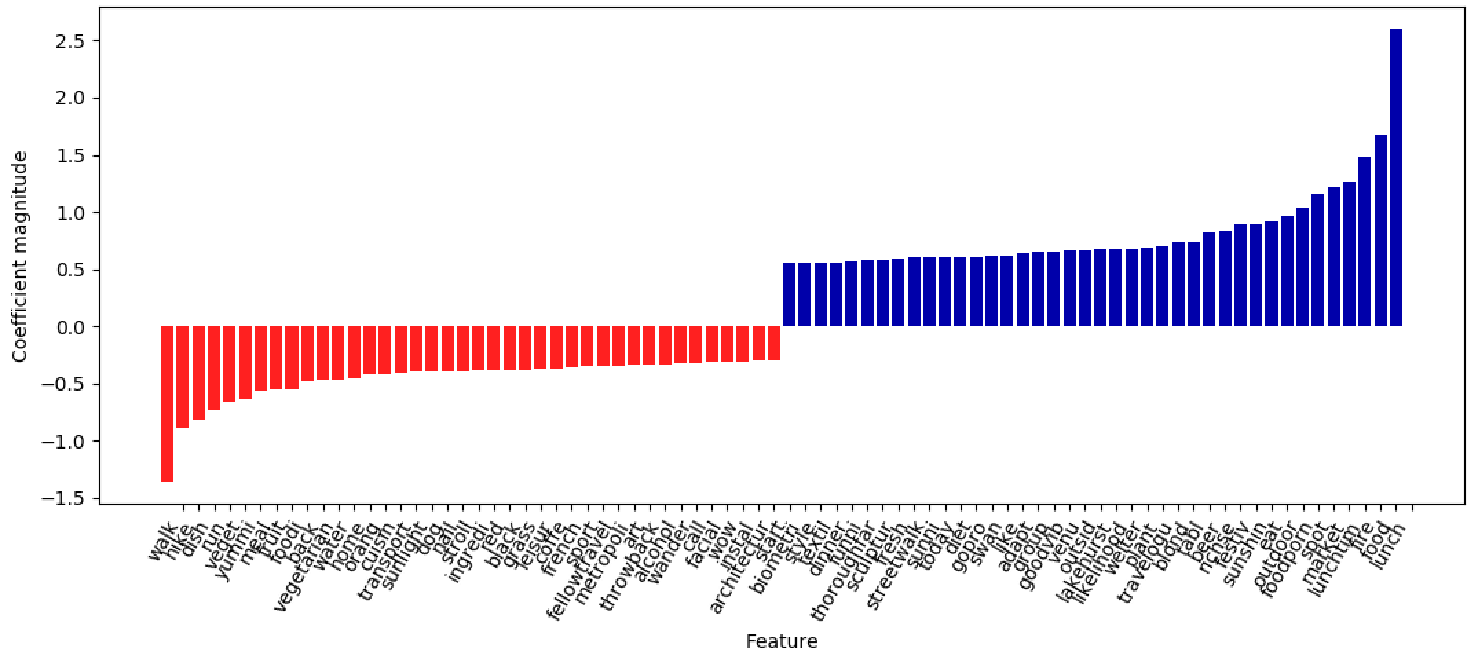
\includegraphics[width=\textwidth]{img/m2_top40_features_picnic_cropped.pdf}
   \caption{The top 80 most predictive M2-features of the class 'picnic'. Blue features are word-tokens which supports the presence of the corresponding classification. Red features support the opposite. The graphic was created with the \textit{mglearn} Python library provided by \textcite{Guido2016}}
   \label{fig:M2_top40_features_picnic}
\end{figure}
\begin{figure}[h!]
   \centering
   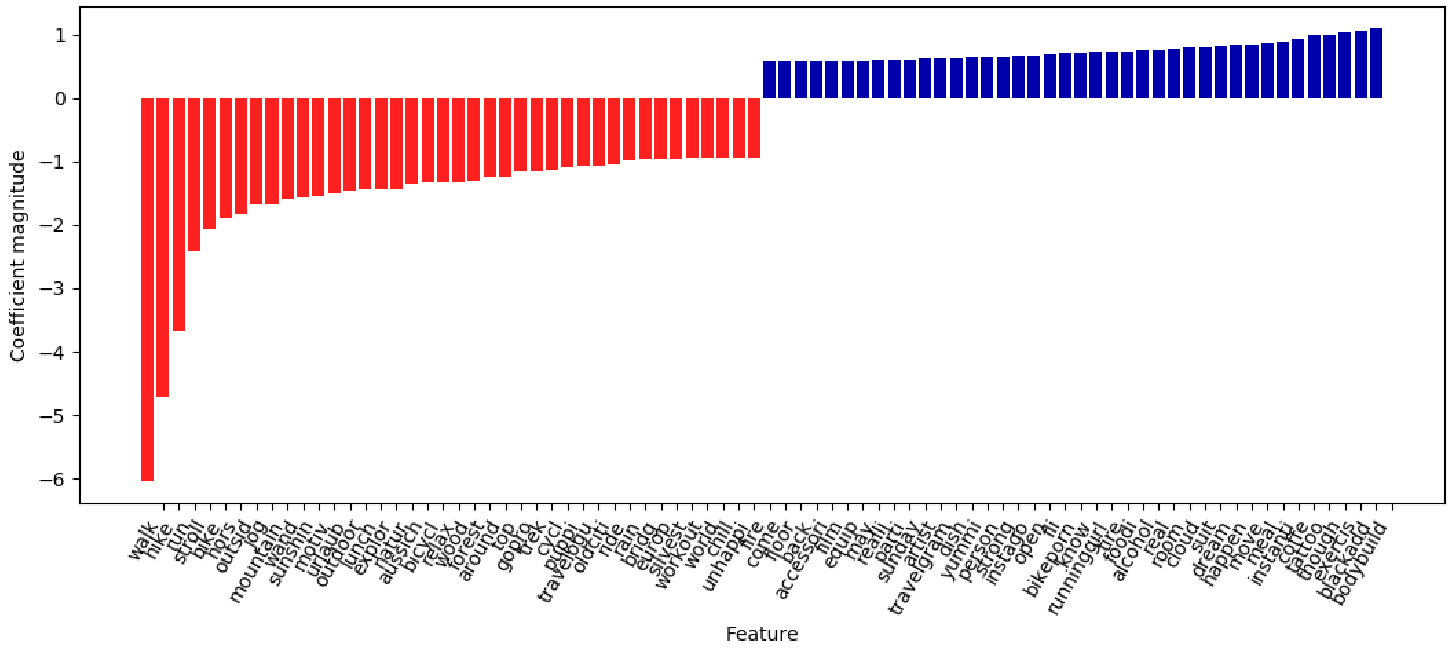
\includegraphics[width=\textwidth]{img/m2_top40_features_None_cropped.pdf}
   \caption{The top 80 most predictive M2-features of the class 'None'. Blue features are word-tokens which supports the presence of the corresponding classification. Red features support the opposite. The graphic was created with the \textit{mglearn} Python library provided by \textcite{Guido2016}}
   \label{fig:M2_top40_features_None}
\end{figure}

\chapter{Interview templates} \label{interview_templates}

\begin{figure}[h!]
   \centering
   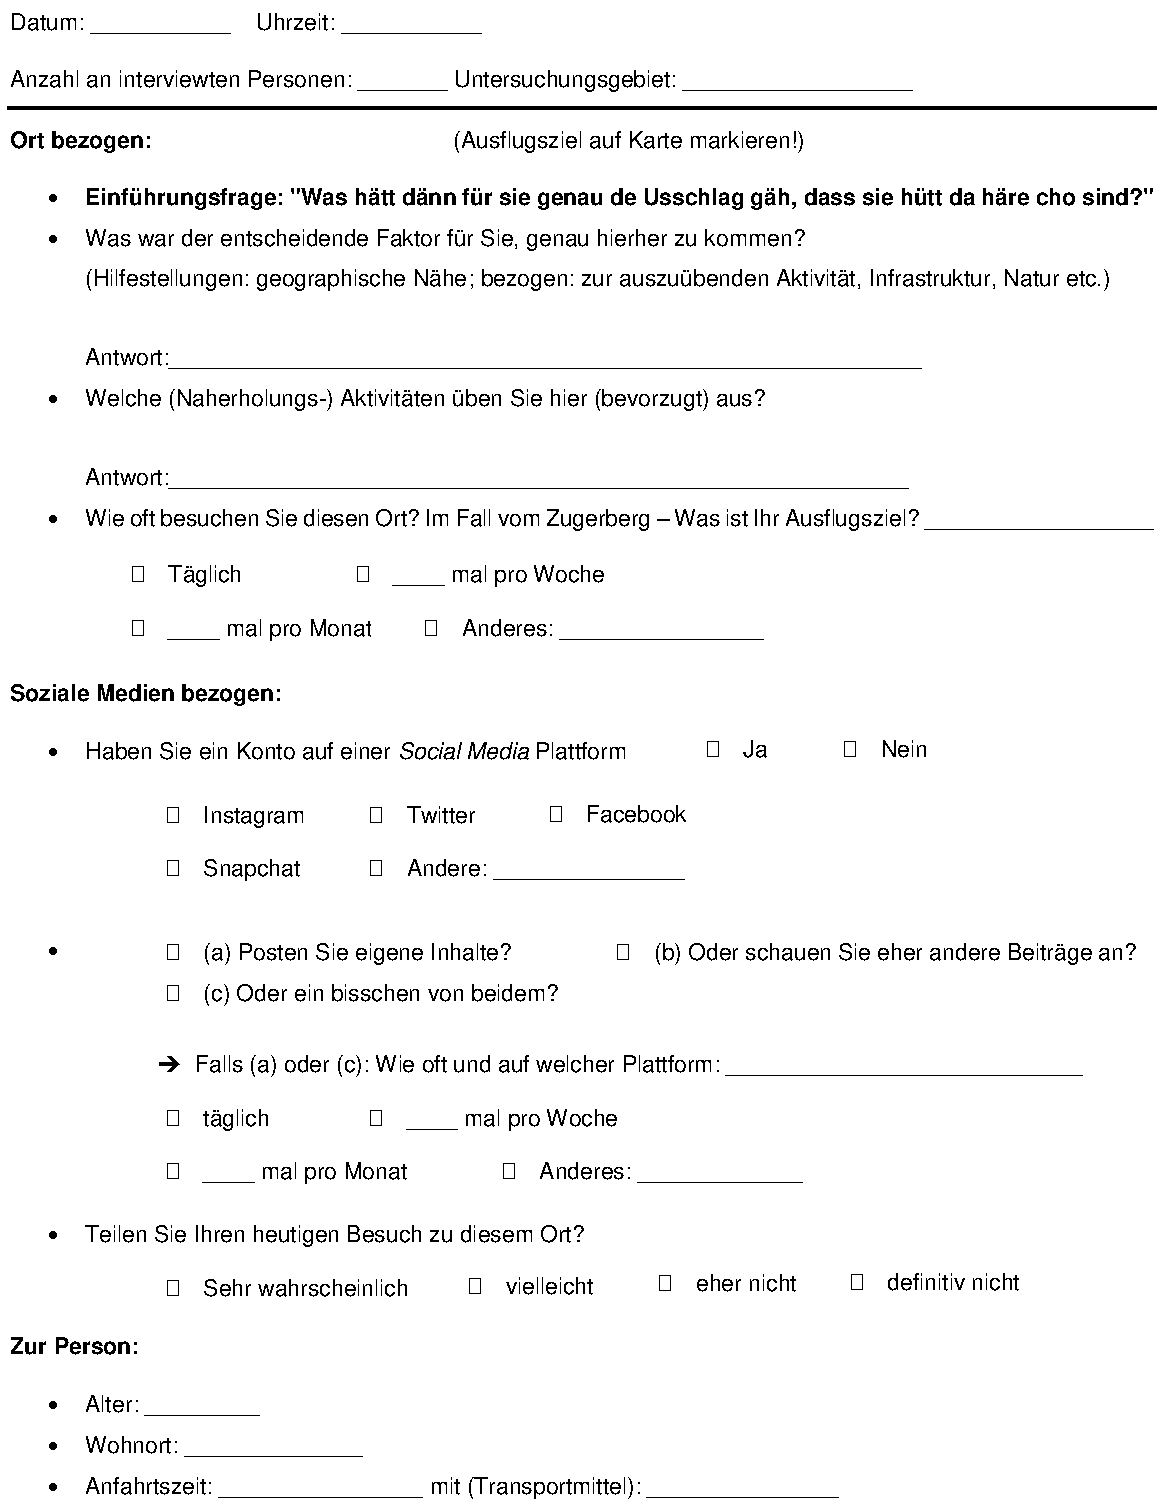
\includegraphics[width=0.8\textwidth]{code/interview_template_cropped.pdf}
   \label{fig:interview_template_appendix}
\end{figure}

\chapter{Passive observation templates} \label{passive_obs_templates}

\begin{figure}[h!]
   \centering
   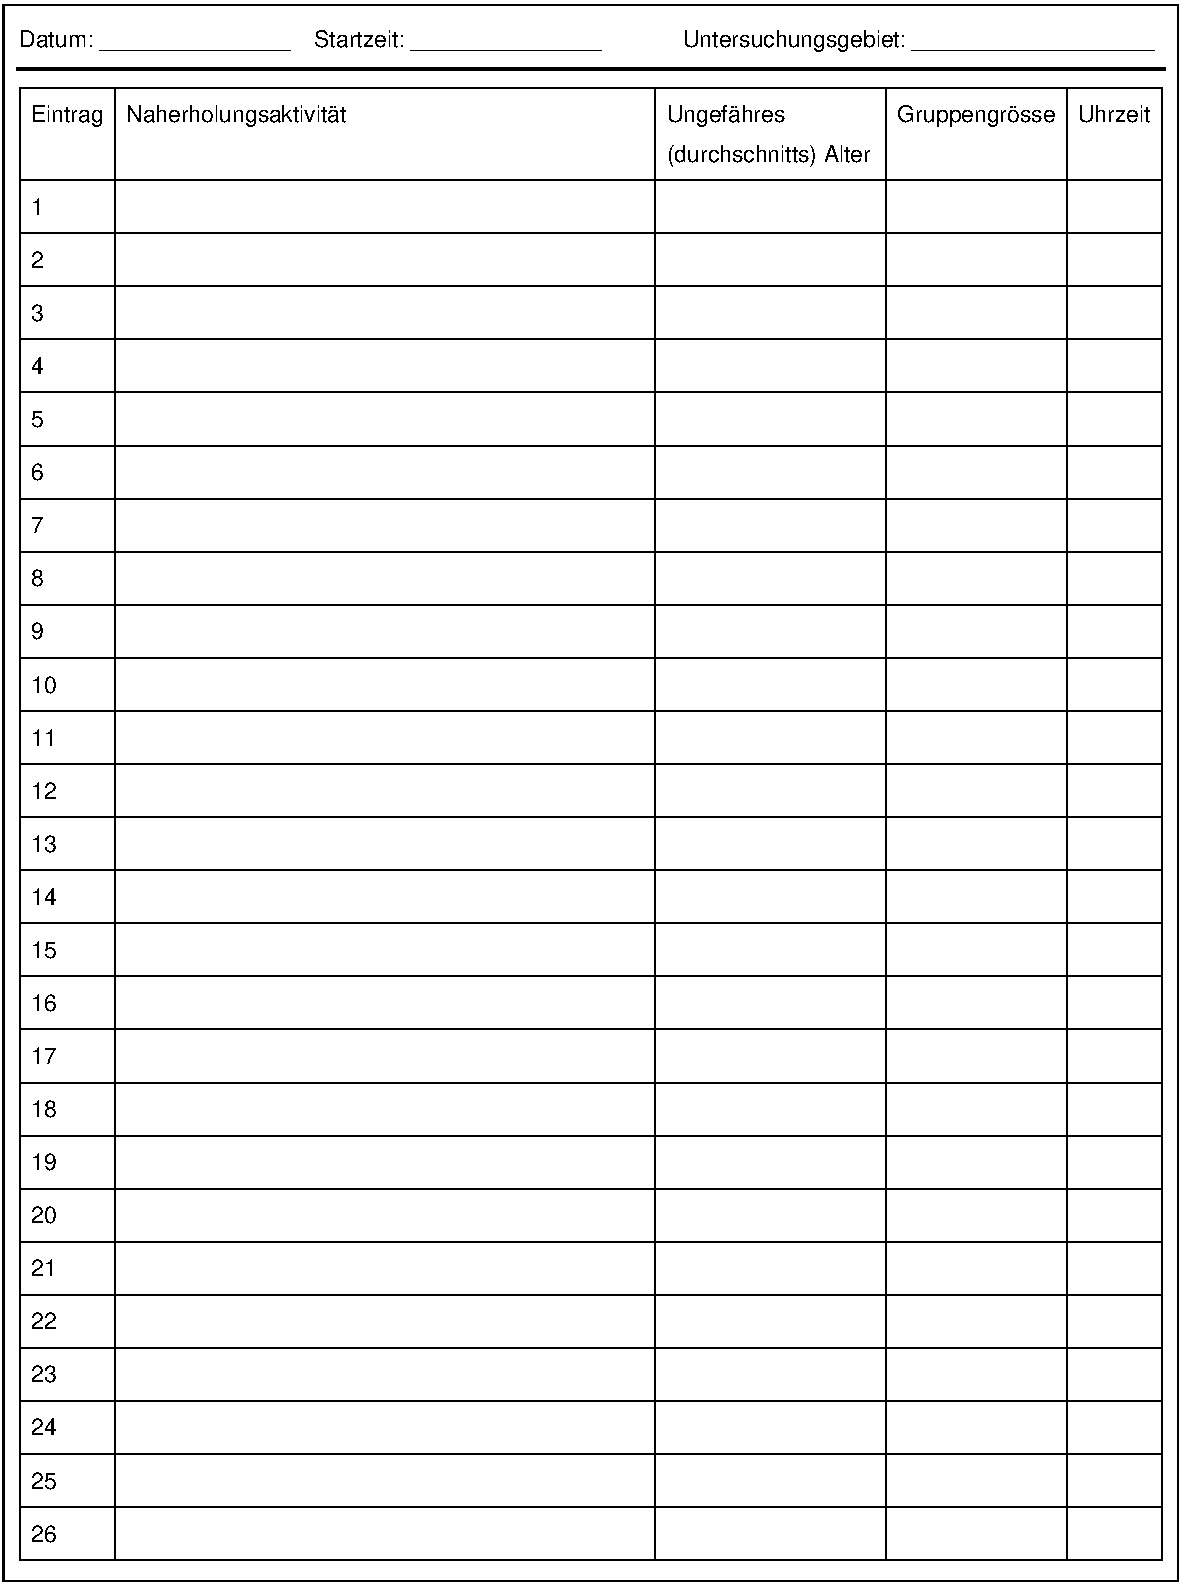
\includegraphics[width=0.8\textwidth]{code/passive_observation_template_cropped.pdf}
   \label{fig:passive_obs_template_appendix}
\end{figure}
